\clearpage
\section{Annexe}
\begin{figure}[ht!]
    \centering
        \begin{subfigure}[b]{0.40\textwidth}
            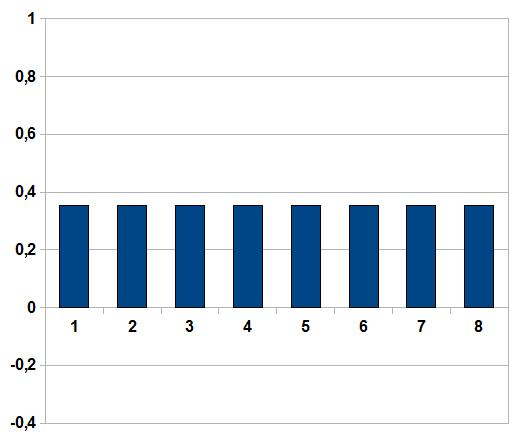
\includegraphics[width=\textwidth]{Grover-EtatInitial.jpg}
            \caption{\footnotesize État initial $|\psi_{(0)}\rangle$}
            \label{fig2:first}
        \end{subfigure}
        \hspace{1cm}
        \begin{subfigure}[b]{0.40\textwidth}
            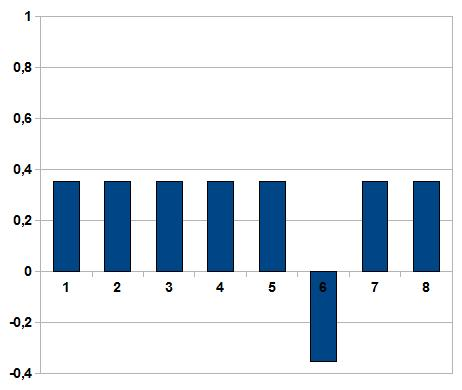
\includegraphics[width=\textwidth]{Grover-PassageParBoiteNoire.jpg}
            \caption{\footnotesize Passage par l'oracle $U_{\omega}$}
            \label{fig2:second}
        \end{subfigure}
        \\
        \begin{subfigure}[b]{0.40\textwidth}
            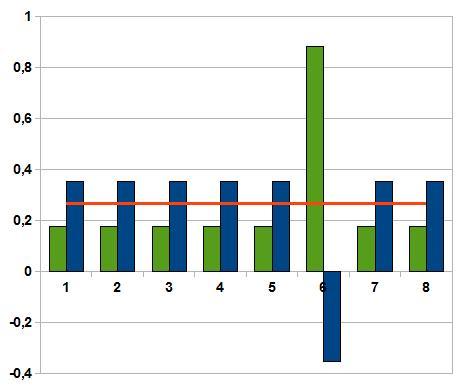
\includegraphics[width=\textwidth]{Grover-MiroirMoyenne.jpg}
            \caption{\footnotesize Passage par l'opérateur de diffusion $U_{\psi}$}\footnotemark
            \label{fig2:third}
        \end{subfigure}
        \hspace{1cm}
        \begin{subfigure}[b]{0.40\textwidth}
            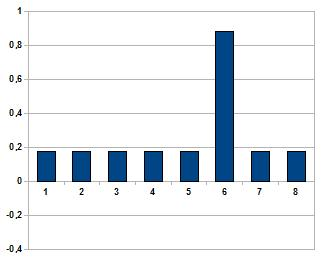
\includegraphics[width=\textwidth]{Grover-Amplification.jpg}
            \caption{\footnotesize État $|\psi_{(1)}\rangle$ résultant après une première iteration}
            \label{fig2:fourth}
        \end{subfigure}
        \\
        \begin{subfigure}[b]{0.40\textwidth}
            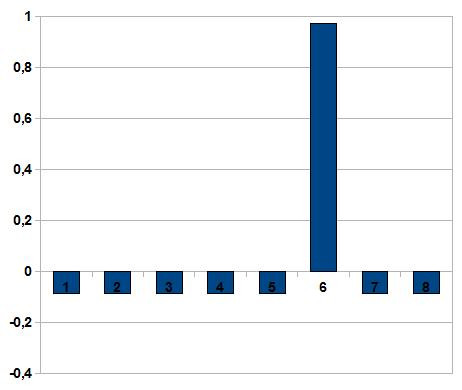
\includegraphics[width=\textwidth]{Grover-EtatFinal.jpg}
            \caption{\footnotesize État final $|\psi_{(r)}\rangle$ maximisant l'amplitude de $|\omega\rangle$ pour $\omega=6$}
            \label{fig2:fifth}
        \end{subfigure}

    \caption{\small Algorithme de Grover pour $\omega=6 \in [\![1,8]\!]$; évolution des amplitudes des vecteurs d'état.}
    \label{fig2:subfigures}
\end{figure}

\footnotetext{La droite rouge correspond à l'amplitude de  $U_{\omega}|\psi_{(0)}\rangle$, et l'histogramme bleu correspond aux amplitudes de chacune de ses composantes. On retrouve les amplitudes des composantes de $|\psi_{(1)}\rangle = U_{\psi}U_{\omega}|\psi_{(0)}\rangle$ avec l'histogramme vert, en remarquant qu'il s'agit d'une symétrie de l'histogramme bleu par rapport à la droite rouge.}
